\chapter{Výsledky}
Zkoumali jsme dvojice molekul $\mathrm{BeH/BeH^-}$ a $\mathrm{OH/OH^-}$, protože se jedná o 
molekuly, které mají vázaný jak základní stav, tak anion, a zároveň se jedná o 
dostatečně malé systémy, aby bylo možné provádět výpočty přesnými metodami.

Ke kvantově chemickým výpočtům jsme používali program MOLPRO.\cite{MOLPRO-WIREs, MOLPRO}. 
Pro určitý soubor mezijaderných vzdáleností\footnote{cca 35 hodnot} jsme napočítali 
energii základního stavu molekuly pro fixovaná jádra, u základního stavu, tak u 
aniontu. Ze znalosti těchto křivek jsme poté zjišťovali parametry molekul, které je 
možné nalézt experimentálně, což jsou disociační energie aniontu i neutrální molekuly a 
elektronové afinity vázané i úplně disociované\footnote{Ta odpovídá odpovídá 
elektronové afinitě některého z prvků v molekule.} molekuly. Protože ale experimentální 
data nejsou určená minimem potenciální energie molekuly, ale základní vibrační 
hladinou, bylo třeba napočítat energetické hladiny dané molekuly. K tomu jsme 
použili metodu výpočtu na na mříži. Vzhledem k počtu geometrií, pro které jsme 
prováděli kvantově-chemické výpočty, který byl nedostatečný pro další numerické výpočty
\footnote{a extrémní výpočetní náročnosti při případném výpočtu v dostatečném počtu 
geometrií}, jsme získané hodnoty proložili kubickým splinem, ze kterého jsme pak 
interpolovali hodnotu potenciálu v několika stovkách bodů. Poté jsme numericky získali 
energetické vibrační hladiny. Toto jsme opakovali pro různé kombinace báze, metoda (, 
aktivní prostor).

\section{BeH}
Základní stav BeH je $^2\Sigma^+$, $\mathrm{BeH}^-$ je pak $^1\Sigma^+$, a v asymptotě 
jdou ke stavům $\mathrm{Be}(^2s) + \mathrm{H}(^2s)$, anion jde pak k $\mathrm{Be}(^2s) + \mathrm{H^-}(^1s)$.

Vyšší stavy jsme neuvažovali, neboť mají jiné asymptotické chování.
při disociaci aniontu pak záporný náboj zůstává na vodíku.\footnote{Berylium má 
zápornou elektronovou afinitu.} Příklady křivek potenciální energie jsou vyobrazeny na obrázku  
\ref{VibrBeH1} spolu se základními vibračními hladinami neutrální molekuly i aniontu.
Křivky v tomto obrázku byly získány metodou FCI v bázi aug-cc-pVTZ.

Podobně jsme  získali elektronovou afinitu molekuly v disociovaném i nedisociovaném 
stavu a disociační energie molekuly i jejího aniontu, které pak můžeme srovnat s 
hodnotami získanými pomocí experimentu. Výsledné hodnoty jsou v tabulce \ref{beh1}

Metodou CI je v tabulkách myšlena metoda MRCI,za níž je uveden použitý aktivní prostor, 
zapsaný počtem jednotlivých molekulových orbitalů v dané ireducibilní reprezentaci pro grupu 
 $C_{2h}$ v pořadí $A_1, B_1, B_2, A_2$. Pro každou metodu je pak za lomítkem uvedena použitá báze.

Experimentální hodnotu disociační energie neutrální molekuly jsme získali 
z \cite{BeH-LeRoy}, její elektronovou afinitu pak z \cite{BeH-ElAf}. Elektronová 
afinita atomárního vodíku je pak známa velmi přesně, 
najít lze například v \cite{H-ElAf}. Disociační energie aniontu jsme 
v literatuře nenalezli, ale dané experimentální hodnoty jsou lineárně závislě, 
lze ji tedy dopočítat pomocí
\begin{equation}
D(\mathrm{AB^-}) = D(\mathrm{AB}) + E_{ea}(B) - E_{ea}(AB),
\end{equation}
za předpokladu, že náboj zůstává na atomu B. Takto získanou hodnotu uvádíme v tabulce v závorce.

Nejnižší získané vibrační hladiny jsou pak v tabulce \ref{beh_vibr}.
\TD přidat experimentální hodnoty (+ citace.)

\begin{figure}
\centering
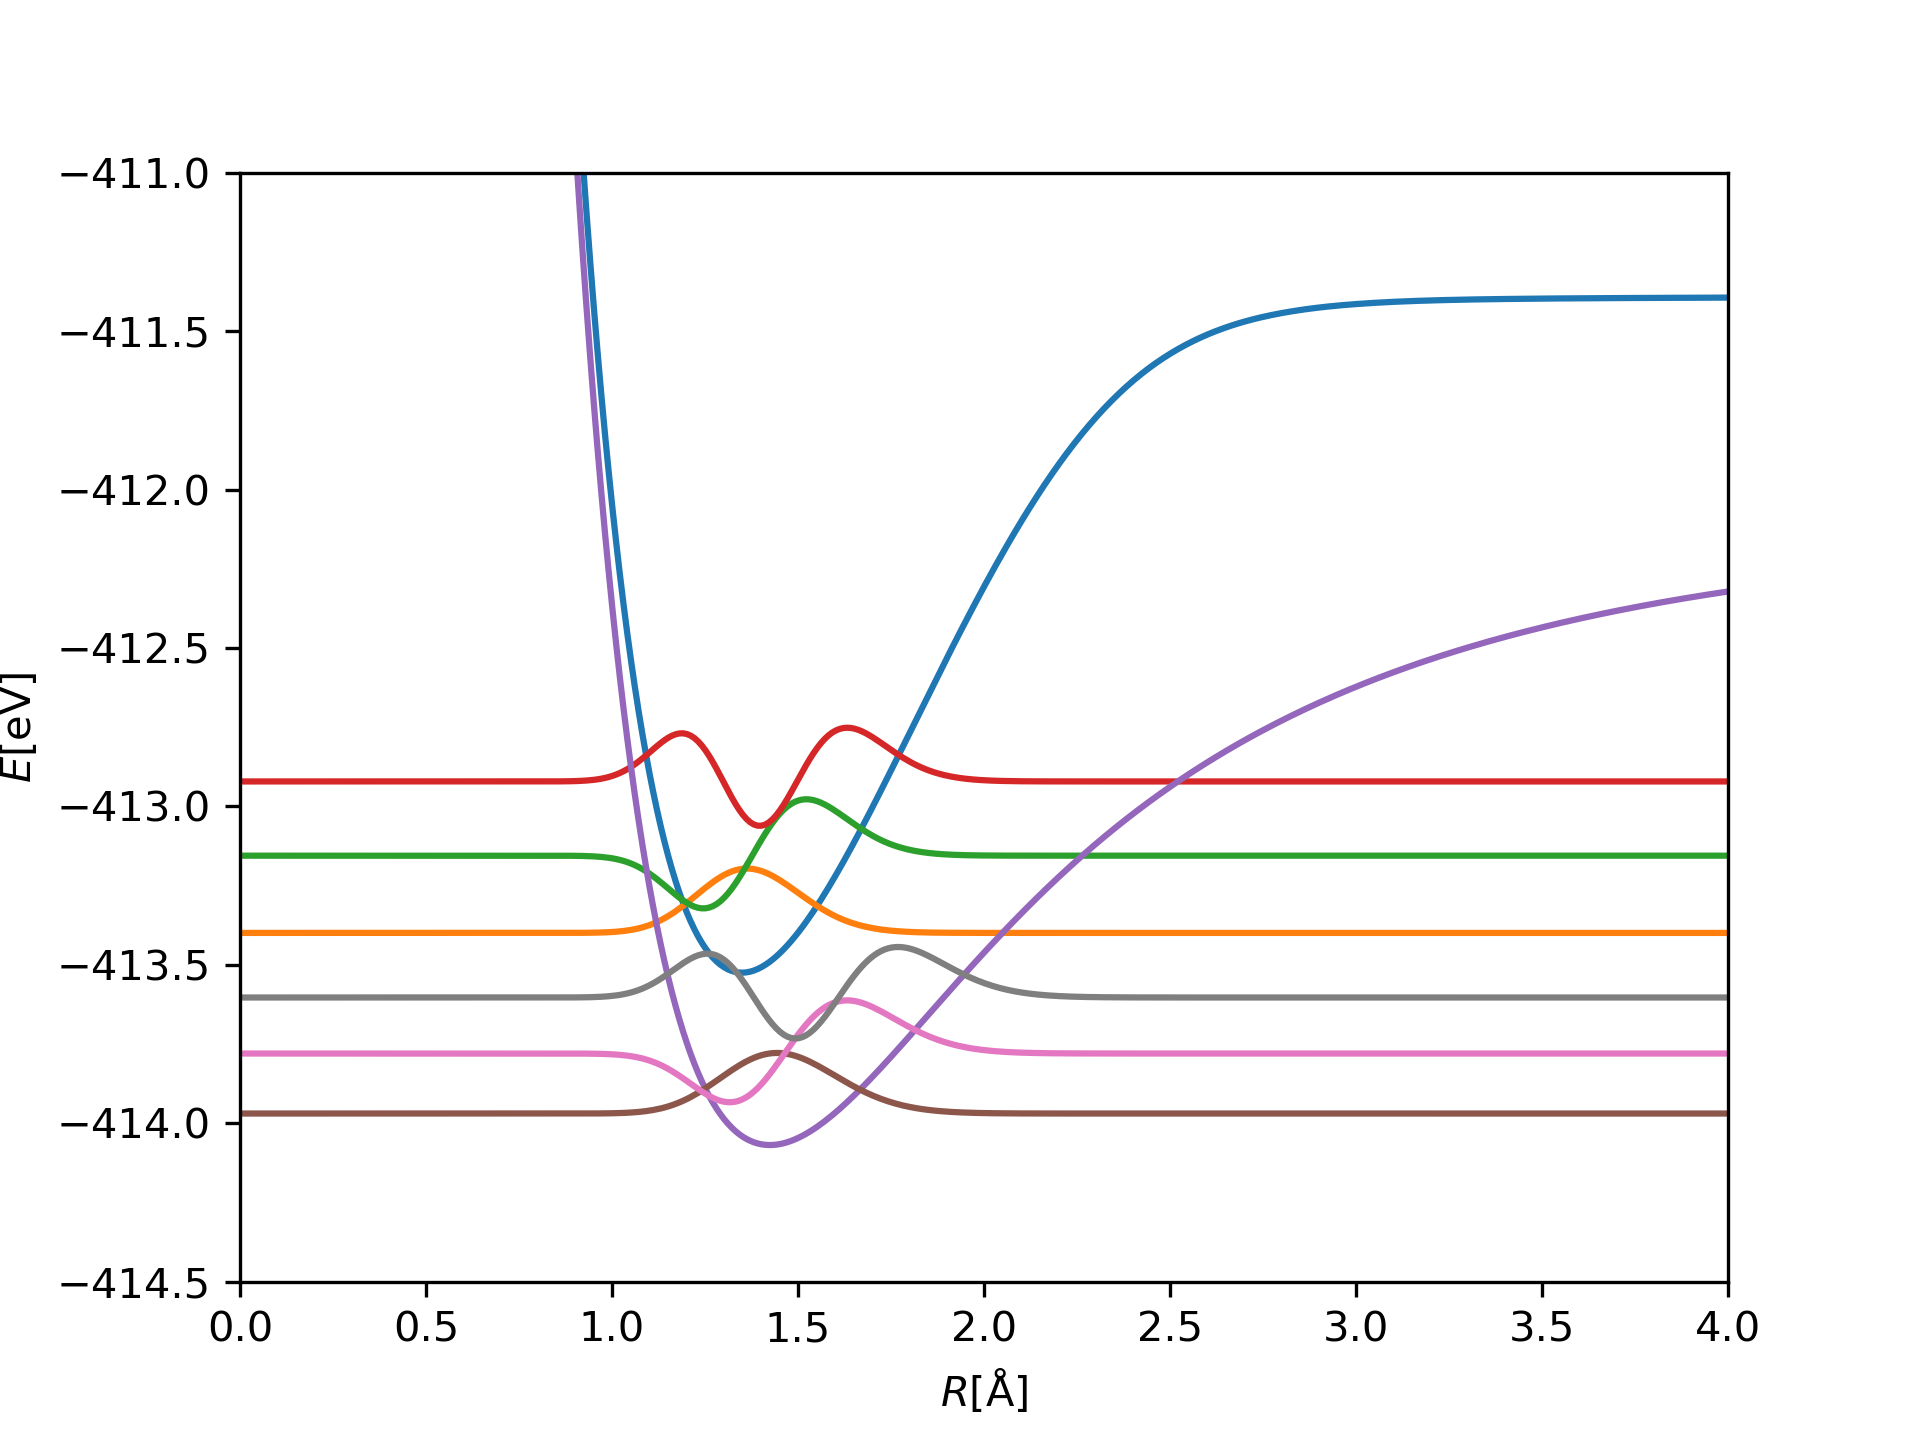
\includegraphics[width=0.8\textwidth]{../img/BeH-vibr1.png}
\caption{Potenciálové křivky základního stavu a nejnižší vibrační hladiny molekul $\mathrm{BeH/BeH^-}$}
\label{VibrBeH1}
\end{figure}
\ltable{../tbl/BeH.tex}{Některé získané měřitelné vlastnosti molekul $\mathrm{BeH/BeH^-}$}{beh1}
\htable{../tbl/BeH-vibr.tex}{Nejnižší čtyři vibrační hladiny molekuly $\mathrm{BeH}$}{beh_vibr}
\section{OH}
Základní stav molekuly OH je $\mathrm{^2\Pi}$ s asymptotou $\mathrm{O}(^3p) + \mathrm{H}(^2s)$. Další stavy jdoucí k této asymptotě jsou $\mathrm{^4\Pi, ^4\Sigma^-, ^2\Sigma^- }$. Anion pak je v základním stavu \TD

Hodnotu disociační energie neutrální molekuly uvádí například \cite{CRC_Handbook90}, stejně jako elektronovou afinitu této molekuly i atomárního kyslíku.
\begin{figure}
\centering
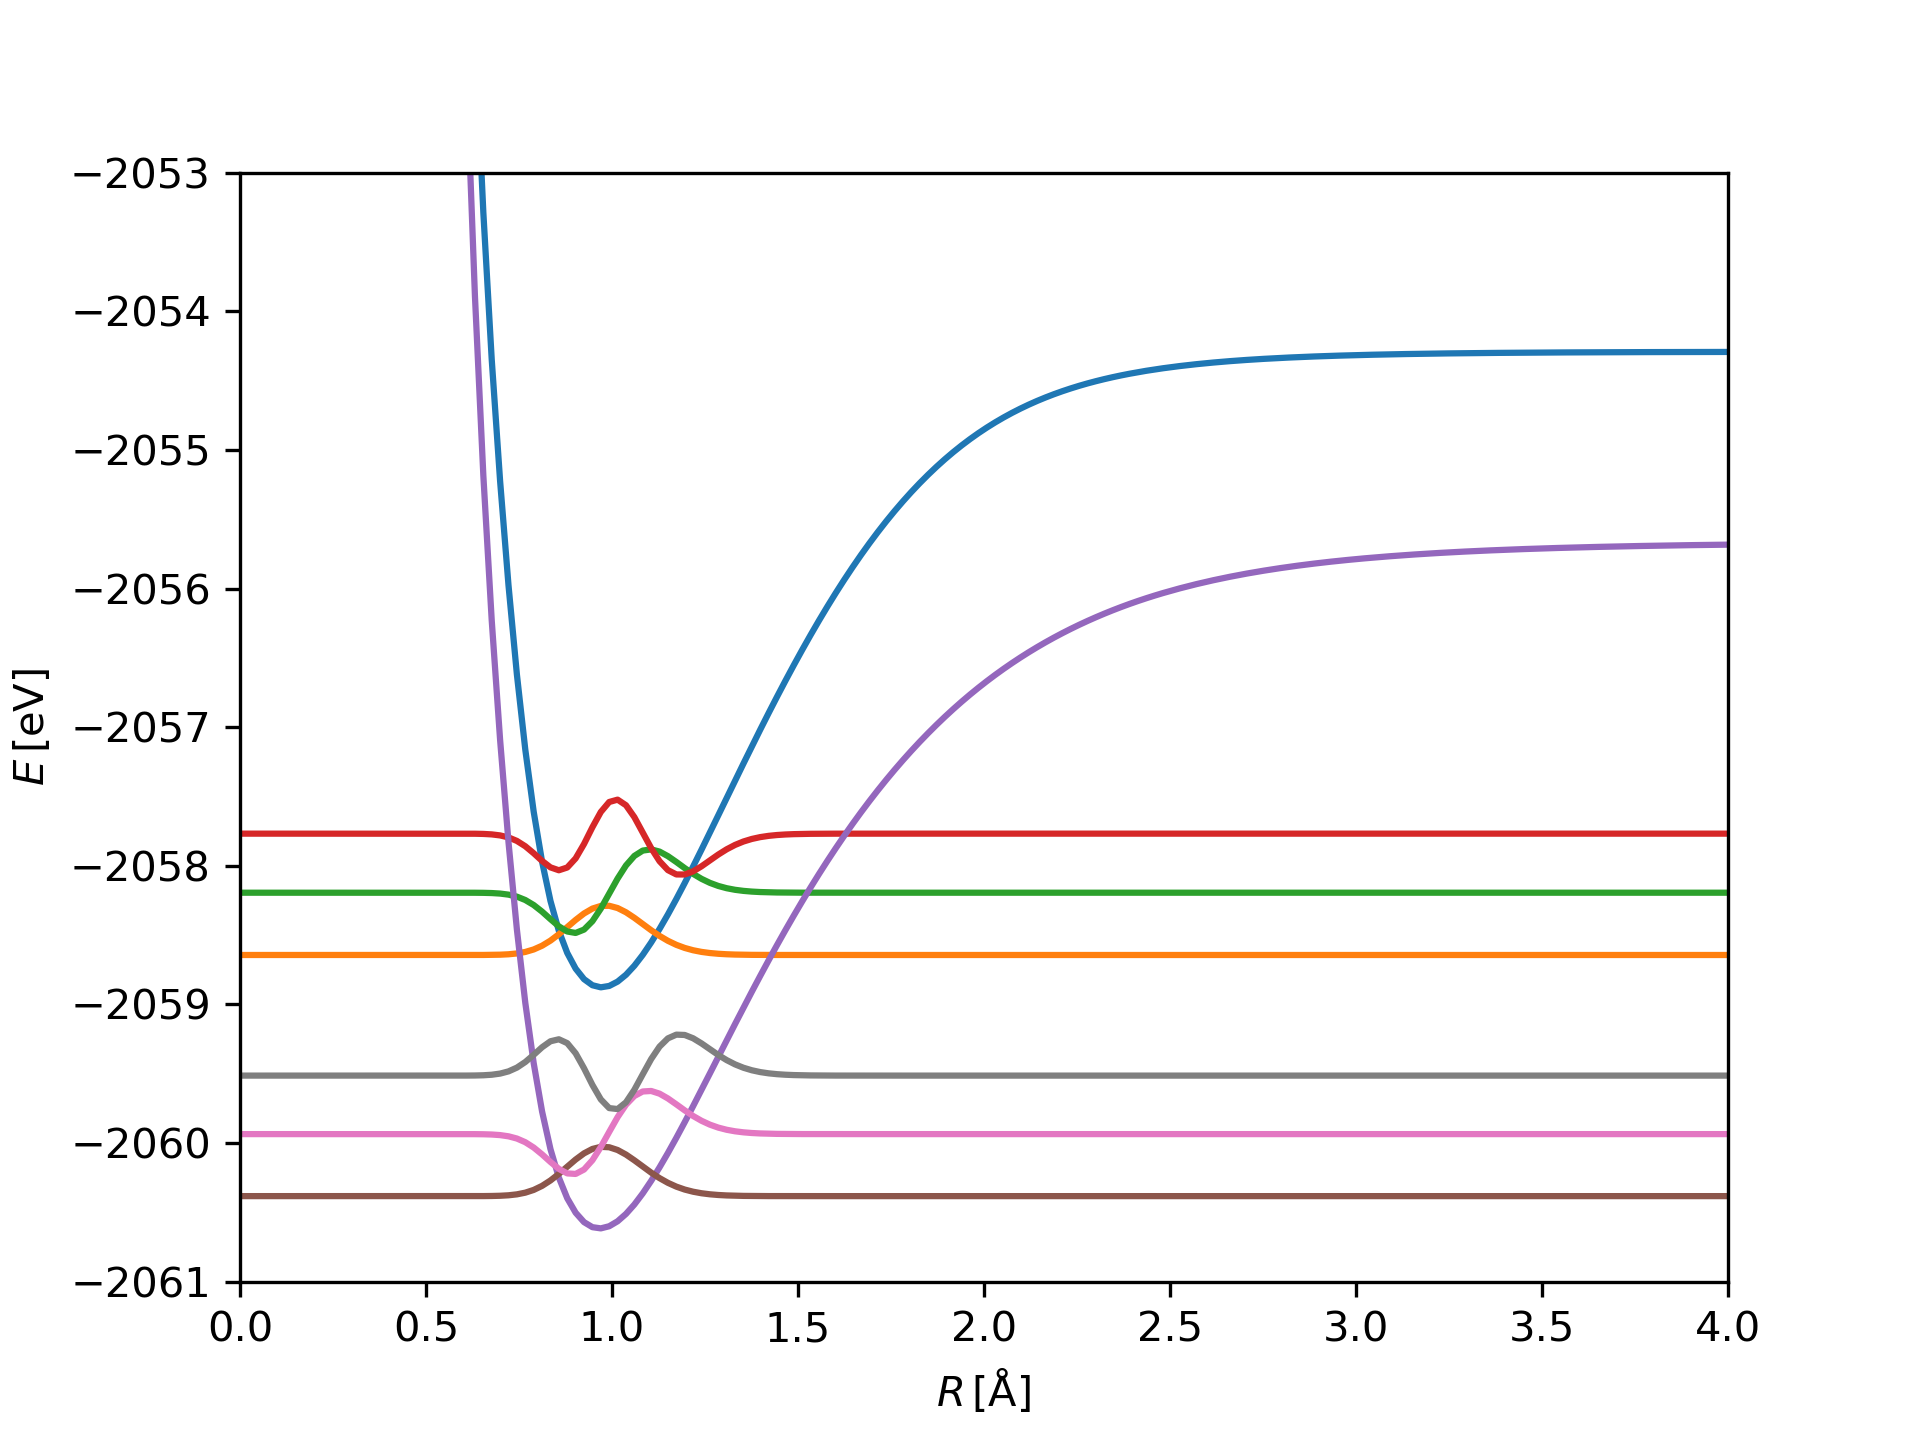
\includegraphics[width=0.8\textwidth]{../img/OH-vibr1.png}
\caption{Potenciálové křivky základního stavu a nejnižší vibrační hladiny molekul $\mathrm{OH/OH^-}$}
\label{VibrOH1}
\end{figure}
\ltable{../tbl/OH.tex}{Některé získané měřitelné vlastnosti molekul $\mathrm{OH/OH^-}$}{oh1}
\htable{../tbl/OH-vibr.tex}{Nejnižší čtyři vibrační hladiny molekuly $\mathrm{OH}$}{oh_vibr}
\htable{../tbl/OHan-vibr.tex}{Nejnižší čtyři vibrační hladiny molekuly $\mathrm{OH^-}$}{ohan_vibr}